\documentclass[conference]{IEEEtran}
\ifCLASSINFOpdf
\else
\fi
\hyphenation{op-tical net-works semi-conduc-tor}

\usepackage[brazilian]{babel}
\usepackage[utf8]{inputenc}
\usepackage[T1]{fontenc}
\usepackage{graphicx}
\graphicspath{ {images/} }

\begin{document}
\title{Avaliação automática de respostas curtas através de uma arquitetura de Deep Learning}


\author{\IEEEauthorblockN{Leonardo Comelli}
\IEEEauthorblockA{ICMC-USP, São Carlos \\
São Paulo, Brasil \\
leonardo.comelli@gmail.com}
}


\maketitle

\begin{abstract}
Com o aumento dos cursos no formato EAD, a avaliação automática de respostas curtas se tornou uma necessidade, visando poupar tempo do professor e diminuindo o tempo de \textit{feedback} para o aluno. Este artigo apresenta, em linhas gerais, alguns artigos que já propuseram uma solução para está tarefa, além de executar uma prova de conceito utilizando \textit{word embeddings} previamente treinadas contra o \textit{corpus} disponibilizado no \textit{SemEval 2013 - Task 7}. O melhor resultado obtido foi uma acurácia de 82,187\%.
\end{abstract}



\IEEEpeerreviewmaketitle



\section{Introdução}
A avaliação de ensino de um aluno esta presente em quase todo o seu período da escolarização, sendo que, em grande parte, esta avaliação é realizada através de questões com respostas curtas. Este modelo de avaliação tem grande relevância, pois avalia a capacidade de leitura, interpretação e criação do aluno. Contudo, o processo de correção manual das respostas exige muito tempo e atenção do professor, além de retardar o \textit{feedback} ao aluno\cite{Santos:2012}.

Com a modernização do sistema de ensino e a crescente oferta de cursos de ensino a distância, que no ano de 2015 ultrapassou a marca dos 2 milhões de alunos\cite{ABED:2015}, a pesquisa por soluções de avaliação automática de respostas esta, cada vez mais, sendo explorada.

Entretanto, o foco em novas soluções para avaliação automática de respostas não deve-se apenas ao crescimento de cursos no formato EAD (Ensino a Distância), a nova geração de processadores (GPU - Graphics Processing Unit) e a utilização de redes neurais multi-camadas (Deep Learning) tem exposto uma série de possibilidades que ainda não haviam sido exploradas.

No sentido de contribuição, este artigo  tem a pretensão de apresentar uma breve revisão sobre o tema e fornecer uma proposta de solução utilizando uma arquitetura de Deep Learning. Além disso, desenvolver uma primeira prova de conceito visando a avaliação automática de respostas curtas de um domínio específico e na lingua inglesa.


\section{Trabalhos Relacionados}
Em meados de 2003, a quantidade de avaliações de ensino e testes preparatórios realizados através da Internet aumentou consideravelmente e a correção automática passou a ser uma necessidade. Nesta época, o foco principal era a avaliação automatizada de redações (TCT\cite{Larkey:1998}, SEAR\cite{Christie:1999}, Intelligent Essay Assessor\cite{Foltz:2003}, IEMS\cite{Ming:2000}, etc), desprezando as questões com respostas curtas que, normalmente, estavam vinculadas aos deveres escolar, avaliações em sala de aula e revisões de capítulos\cite{Leacock:2003}.

Aproveitando essa lacuna e entendendo a necessidade de avaliar automaticamente as questões com respostas curtas a Educational Testing Service(ETS) Technologies, empresa especializada em aplicação e correção de testes para diversas instituições, desenvolveu o c-Rater. Uma ferramenta específica para respostas curtas que difere, em muitos pontos, das ferramentas existentes (na época) focadas em avaliação automatizada de redações\cite{Leacock:2003}.

Ainda em 2003, o UCLES Group (Cambridge-ESOL, Cambridge International Examinations e Oxford, Cambridge and RSA Examinations) que provê serviços de avaliação ao redor do mundo iniciou o desenvolvimento do OXFORD-UCLES, que utilizava técnicas similares ao c-Rater para garantir um processamento eficiente frente a dados com ruídos (erros gramaticais ou ortográficos). As técnicas de extração de informações baseadas em padrões foram amplamente utilizadas contra 201 questões de biologia retiradas do General Certificate of Secondary Education, obtendo a acurácia de 88\% \cite{Sukkarieh:2003}.

Passado algum tempo, a ETS Technologies publicou algumas evoluções no c-Rater, como a utilização de conceitos: onde, dado um conceito \textit{C} e uma resposta de aluno \textit{A}, ele verifica se \textit{C} é uma inferência ou esta parafraseando \textit{A} (em outras palavras, se A implica C então A é verdadeiro)\cite{Sukkarieh:2009}. O experimento realizado neste artigo, utilizou 12 questões de respostas curtas em inglês (7 compreensão de texto e 5 matemática) retiradas de um exame aplicado em alunos da 7ª e 8ª série. As questões foram previamente corrigidas e pontuadas por dois humanos, sendo que o melhor resultado das médias entre o c-Rater e cada humano (c-H1 / H2) foi 98\%.

Embora a língua mais utilizado nas pesquisas seja a inglesa, existem alguns artigos publicados voltados para outras linguas, como por exemplo a língua portuguesa, que foi utilizada em uma pesquisa para avaliação automática de respostas discursivas  utilizando um método LSA (Latent Semantic Analysis)\cite{Sukkarieh:2009}. Os testes para avaliar a eficiência desta proposta foram realizados a partir de amostras do corpus fornecido pela Universidade Federal do Pará, sendo: 130 questões de Biologia e 229 de Geografia. Visando garantir os melhores resultados, foi utilizado um modelo de regressão linear múltipla para cada disciplina, obtendo a acurácia de 85,62\% para Biologia e 87,35\% para Geografia.

\section{Proposta}
Esta pesquisa, tem como objetivo principal, verificar a eficiência da utilização de uma arquitetura Deep Learning na correção automática de respostas curtas. O fluxo da arquitetura proposta contém algumas etapas de pré-processamento (corretores), onde o foco será a eliminação de ruídos e uma manipulação eficiente dos dados, considerando que os dados fornecidos por alunos são, na maioria das vezes, constituídos por erros de ortografía e gramática. Este fluxo está representado na Figura 1.

Neste momento, o inutito é validar a acurácia da classificação textual baseada em \textit{word embeddings} previamente treinadas. Por este motivo, o \textit{corpus} utilizado para a validação foi estruturado e manipulado de antemão em outra pesquisa. O corpus em questão é o \textit{SemEval 2013 - Task 7}\cite{Dzikovska:2013} que será detalhado posteriormente.


\subsection{Arquitetura}

\begin{figure}[h]
\centering
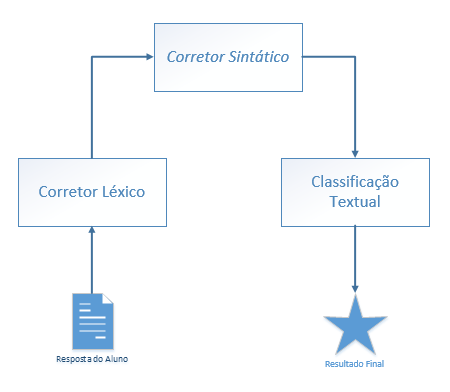
\includegraphics[width=0.5\textwidth]{arquitetura}
\caption{Arquitetura: Fluxo proposto}
\end{figure}


A entrada para o fluxo é a resposta do aluno que, primeiramente, deve passar pela etapa de correção léxica para detectar os erros de grafia. Para auxiliar na execução dessa etapa, uma sugestão de ferramenta é o Stanford Parser \cite{StanfordParser:2005}, que foi desenvolvimento dentro do \textit{The Stanford Natural Language Processing Group} e pode ser utilizado com a língua portuguesa, além de possuir suporte a diversas linguagens de programação. 

Na etapa seguinte, a correção sintática é executada para detectar os erros em relações entre as palavras. Para essa etapa a sugestão é a ferramenta CoGrOO \cite{CCSL:2013}, que é um corretor gramatical acoplável ao \textit{LibreOffice} desenvolvido pelo Centro de Competência em Software Livre do IME/USP. 

As ferramentas citadas para auxiliar nas etapas de correção possuem uma série de implementações prontas, porém é evidente que será necessário algum tipo de evolução para garantir uma maior eficiência dentro no domínio pesquisado. Os corretores (léxico e sintático) são importantes para diminuir os ruídos para as etapas subsequentes.

A última etapa da arquitetura é a principal, onde o esforço em validar a proposta foi concentrado. O objetivo dessa etapa é garantir que uma resposta correta de um aluno seja similar a resposta referência e uma resposta incorreta não tenha esta similaridade, baseado na definição de \textit{Textual Entailment} onde: um texto T implica em outro texto H, se H é tido como verdade em todas as circunstâncias nas quais T é verdade \cite{Dagan:2006}.

Para esta etapa é necessário uma ferramenta que consiga medir a similaridade entre a resposta do aluno e uma ou mais respostas-referência. A opção escolhida para a prova de conceito foi o Doc2Vec \cite{Mikolov:2016} que utiliza \textit{word embeddings} treinadas previamente contra as respostas-referência e/ou corretas para realizar a classificação textual. 

O resultado esperado ao término da execução do fluxo é o quão uma resposta de um aluno é similar a uma resposta referência, esta similaridade é representada por uma porcentagem.

\subsection{Corpus}
O \textit{corpus} utilizado para a validação da proposta foi o disponibilizado no \textit{SemEval 2013 - Task 7}\cite{Dzikovska:2013}. Este corpus, na sua totalidade,  é composto por 56 questões sobre eletricidade/eletrônica com 3000 respostas e 197 questões de 15 domínios variados com 10000 respostas, todas as perguntas e respostas estão na língua inglesa. As respostas estão classificadas em: \textit{5-way} (correta, parcialmente correta, contraditória, irrelevante e fora do domínio), \textit{3-way} (correta, contraditória e incorreta) e \textit{2-way} (correta e incorreta).

\begin{figure}[h]
\centering
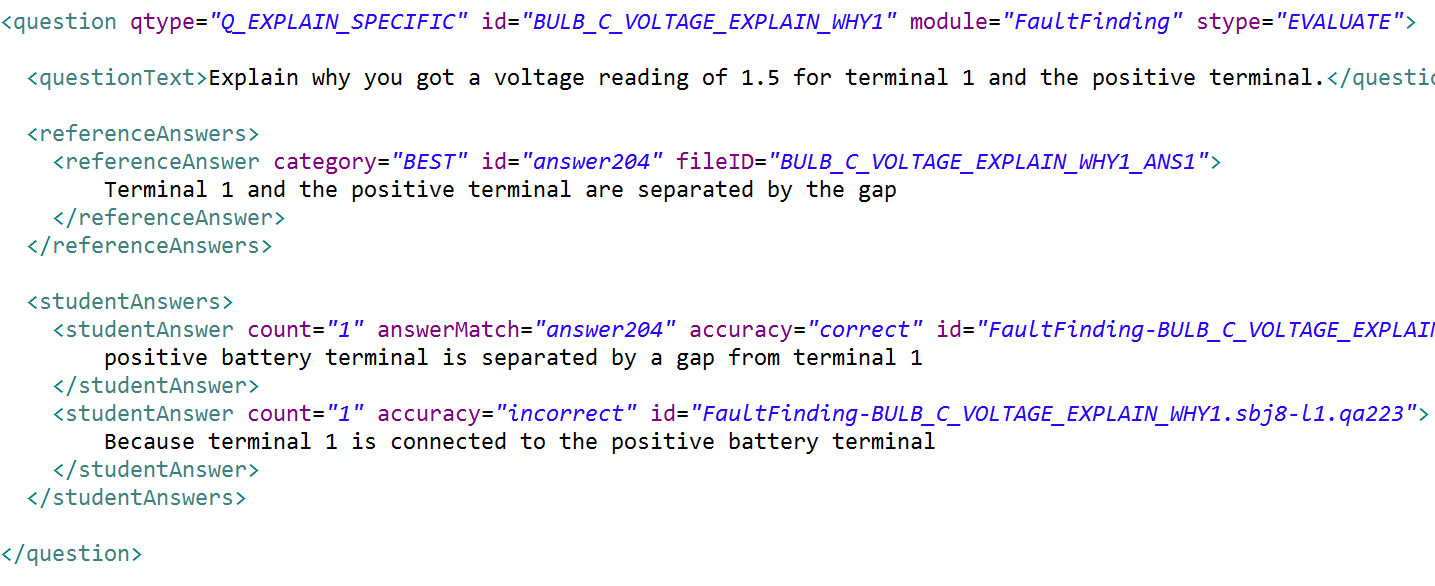
\includegraphics[width=0.5\textwidth]{corpus}
\caption{Corpus: SemEval 2013 - Task 7 - Formato XML}
\end{figure}

Para a validação da prova de conceito foi retirado uma amostra das questões sobre eletricidade/eletrônica, sendo: 1 questão com 151 respostas classificadas no \textit{2-way} (correta e incorreta). Para facilitar a execução, a amostra das questões que serão utilizadas foram convertidas do formato XML (conforme Figura 2) para dois arquivos no formato texto, onde um contêm apenas as questões corretas e o outro as incorretas (apresentado na Figura 3).

\begin{figure}[h]
\centering
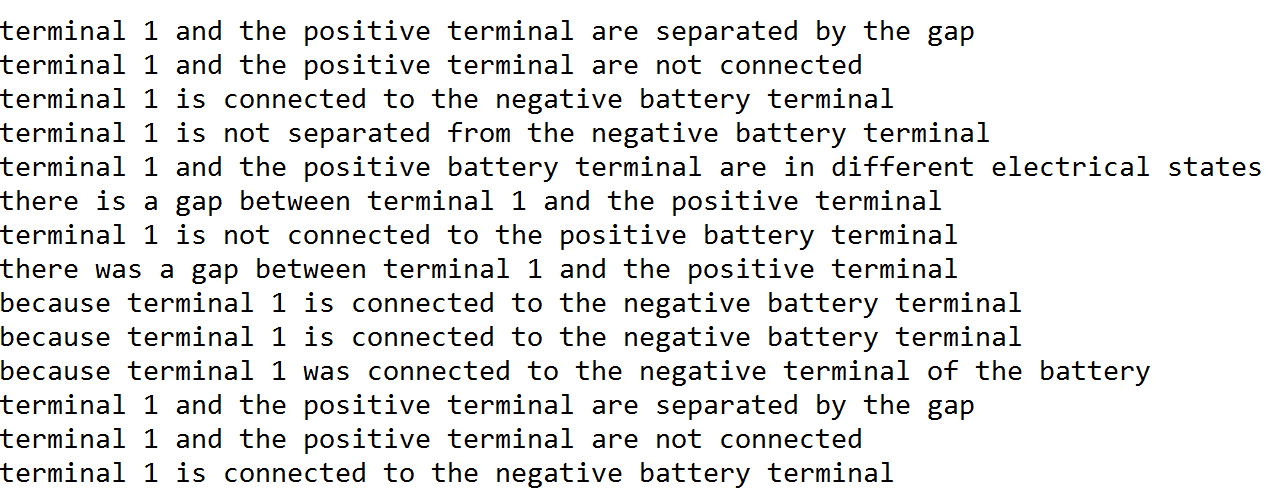
\includegraphics[width=0.5\textwidth]{corpus_txt}
\caption{Corpus: SemEval 2013 - Task 7 - Formato TXT}
\end{figure}

O corpus completo do \textit{SemEval 2013 - Task 7} esta disponível na internet de forma pública \cite{DzikovskaCorpus:2013}, assim como a amostra retirada para a validação da proposta \cite{Comelli:2016}.

\subsection{Implementação}
A prova de conceito foi implementada com o apoio de alguns bibliotecas \textit{python} que auxiliam o desenvolvimento de soluções de Processamento de Linguagem Natural, com destaque para o \textit{gensim} \cite{gensim:2016} que possui uma implementação do Doc2Vec e o \textit{scikit-learn} \cite{sklearn:2016} que disponibiliza uma série de algoritmos para análise dados.

\begin{figure}[h]
\centering
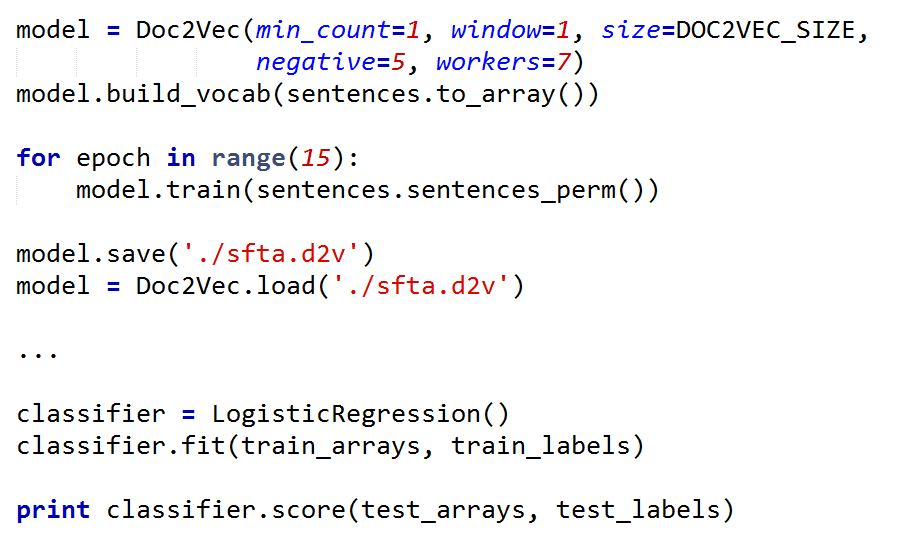
\includegraphics[width=0.5\textwidth]{code}
\caption{Implementação: Trecho do código}
\end{figure}

Os exemplos disponibilizados no site do \textit{gensim} foram a base para o desenvolvimento, conforme trecho de código apresentado na Figura 4. A maior parte do \textit{corpus} foi utilizada para o treino e o restante para a realização dos testes. Buscando assegurar uma maior qualidade nos resultados obtidos, foram executados diversos testes sobre o mesmo corpus, sempre construindo os fragmentos de treino e teste de forma aleatória.

Ao final de cada execução, com o suporte da biblioteca \textit{scikit-learn}, uma regressão logística é calculada com o intuito de tornar os resultados mais apurados.

Todos os artefatos desenvolvidos foram disponibilizados publicamente na internet \cite{Comelli:2016}.


\section{Resultados}
O resultado foi obtido diante de um \textit{corpus} com 151 respostas únicas, sendo que 135 foram utilizadas para treino e 16 para os testes. Para aumentar o tamanho do \textit{corpus}, foram realizadas 10 iterações sobre o mesmo, separando os fragmentos de teste e treino de aleatória na mesma proporção citada anteriormente, totalizando 1600 testes.

A primeira validação da proposta atingiu a acurácia de 82\%, conforme mostrado na Tabela I. Embora o resultado esteja abaixo de outras pesquisas, é importante ressaltar a arquitetura enxuta e o \textit{corpus} com poucos ruídos.

\begin{table}[h]
\caption{Resultados - Acurácia: Testes com Doc2Vec}
\centering
\begin{tabular}{ccc}
\textbf{Testes}                   & \textbf{Acertos}                  & \textbf{Acurácia \(\%\)} \\ \hline
160                                     & 132                                      & 82,500          \\
160                                     & 135                                      & 84,375          \\
160                                     & 130                                      & 81,250          \\
160                                     & 129                                      & 80,625          \\
160                                     & 130                                      & 81,250          \\
160                                     & 130                                      & 81,250          \\
160                                     & 126                                      & 78,750          \\
160                                     & 138                                      & 86,250          \\
160                                     & 133                                      & 83,125          \\
160                                     & 132                                      & 82,500          \\ \hline
\textbf{1600}                     & \textbf{1315}                        & \textbf{82,187}  \\ \hline
\end{tabular}
\end{table}

Comparando os resultados com outras pesquisa (vide Figura 5), fica evidente a proximidade dos resultados e possibilidade de melhorar, significativamente, os resultados obtidos na primeira prova de conceito no decorrer da pesquisa.

\begin{figure}[h]
\centering
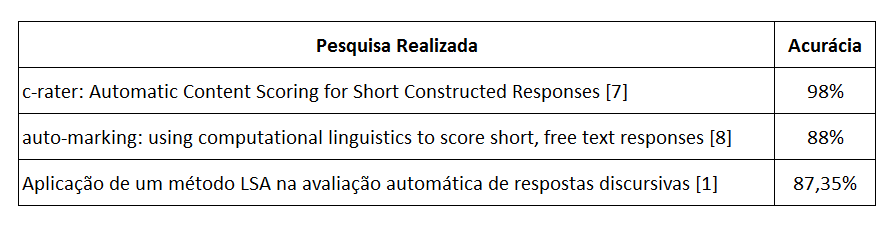
\includegraphics[width=0.5\textwidth]{outras_pesquisas}
\caption{Resultados: Comparação com outras pesquisas}
\end{figure}

\section{Conclusão}
O foco deste artigo foi a avaliação automática de respostas curtas, demonstrando de forma prática a possibilidade de validar a similaridade entre a resposta do aluno e uma ou mais respostas-referência utilizando técnicas de \textit{word embeddings} através do Doc2Vec. Durante a pesquisa, notou-se que a similaridade entre respostas curtas pode ser muito sensível dependendo do domínio e os resultados podem, em alguns casos, conter "falso-verdadeiro".

Os resultados obtidos não estão acima do estado da arte para a tarefa proposta, porém são satisfatórios e importantes para a evolução da arquitetura apresentada.

\section{Trabalhos Futuros}
Os próximos passos serão a execução de testes utilizando o \textit{corpus} da plataforma de ensino chamado Alura \cite{Alura:2016}, onde o domínio principal é a área de tecnologia e programação. Esta plataforma possui 232 cursos, 1734 aulas e 8170 questões na lingua portuguesa; sendo que já foi liberado para testes iniciais uma amostra com 06 questões e mais de 7000 respostas. Provavelmente a mudança de idioma implicará em alguns ajustes nas etapas previstas e, até mesmo, a inclusão de novas.

Além do trabalho com outro \textit{corpus}, esta previsto o estudo de redes neurais multi-camadas, como por exemplo: LSTM \cite{SkymindLSTM:2016} e/ou CNN \cite{SkymindCNN:2016}, em conjunto com as \textit{word embbedings}.

Como objetivo secundário, todos os artefatos serão sempre disponibilizados como código aberto para a comunidade, exceto as informações disponibilizados por terceiros em caráter confidencial.


\section*{Agradecimentos}
Em especial à professora Dra. Sandra Aluísio do curso Tópicos em Inteligência Artificial do ICMC/USP e a todos os colegas da turma por compartilhar o conhecimento que foi vital para a confecção deste artigo.


\begin{thebibliography}{1}

\bibitem{Santos:2012}
João Carlos Alves dos Santos, Tácio Ribeiro, Eloi Favero, Joaquim Queiroz, [2012], \emph{"Aplicação de um método LSA na avaliação automática de respostas discursivas."}, Anais do Workshop de Desafios da Computação Aplicada à Educação.

\bibitem{ABED:2015}
ABED – Associação Brasileira de Educação a Distância, \emph{"Censo EAD Brasil
2014, 2015"}. Disponível em: http://www.abed.org.br/censoead2014, acessado em: junho de 2016.

\bibitem{Larkey:1998}
Larkey, L., [1998], \emph{"Automatic essay grading using text categorization
techniques."}, In In proceedings of the 21st annual international ACM SIGIR Conference on Research and Development in Information Retrieval.

\bibitem{Christie:1999}
Christie, J. [1999], \emph{"Automated essay marking for both content and style."}, In Proceedings of the 3rd International Computer Assisted Assessment Conference.

\bibitem{Foltz:2003}
Foltz, P.; Laham, D.; and Landauer, T. [2003], \emph{"Automated essay scoring."}, In Applications to educational technology.

\bibitem{Ming:2000}
Ming, Y.; Mikhailov, A.; and Kuan, T. L. [2000], \emph{"Intelligent
essay marking system."}, Technical report, Learner Together NgeANN Polytechnic, Singapore.

\bibitem{Leacock:2003}
Leacock, C., and Chodorow, M., [2003], \emph{"C-rater: Automated
scoring of short-answer questions."}, Computers and Humanities, 389–405.

\bibitem{Sukkarieh:2003}
Sukkarieh, J. Z.; Pulman, S. G.; and Raikes, N., [2003], \emph{"Auto-marking: using computational linguistics to score short, free text responses."}, In Presented at the 29th IAEA.

\bibitem{Sukkarieh:2009}
Sukkarieh, Jana Zuheir, and John Blackmore, [2009], \emph{"c-rater: Automatic Content Scoring for Short Constructed Responses."}, FLAIRS Conference.

\bibitem{Dzikovska:2013}
Dzikovska, M. O., Nielsen, R. D., Brew, C., Leacock, C., Giampiccolo, D.,
Bentivogli, L., ... \& Dang, H. T, [2013], \emph{"SemEval-2013 task 7: The joint student response analysis and 8th recognizing textual entailment challenge."}, NORTH TEXAS STATE UNIV DENTON.

\bibitem{StanfordParser:2005}
The Stanford Natural Language Processing Group, \emph{"The Stanford Parser: A statistical parser"}, Stanford University. 2005. Disponível em: http://nlp.stanford.edu/software/lex-parser.html, acessado em: agosto de 2016.

\bibitem{CCSL:2013}
CCSL - Centro de Competência em Software Livre, \emph{"CoGrOO – Corretor Gramatical acoplável ao LibreOffice"}, IME - USP. 2013. Disponível em: http://cogroo.sourceforge.net, acessado em: junho de 2016.

\bibitem{Dagan:2006}
Dagan, I., Glickman, O. e Magnini, B., [2006], \emph{"The PASCAL Recognising Textual Entailment Challenge"}, Proceedings of the First International Conference on Machine
Learning Challenges: Evaluating Predictive Uncertainty Visual Object Classifi-
cation, and Recognizing Textual Entailment.

\bibitem{Mikolov:2016}
Quoc V. Le, Tomas Mikolov, \emph{"Distributed Representations of Sentences and Documents"}, 2016. Disponível em: http://arxiv.org/abs/1405.4053, acessado em: agosto de 2016.

\bibitem{DzikovskaCorpus:2013}
Dzikovska, M. O., Nielsen, R. D., Brew, C., Leacock, C., Giampiccolo, D.,
Bentivogli, L., ... \& Dang, H. T, \emph{"SemEval-2013 task 7: The joint student response analysis and 8th recognizing textual entailment challenge."}, 2013. Disponível em: https://www.cs.york.ac.uk/semeval-2013/task7/index.php\%3Fid=data.html, acessado em: agosto de 2016.

\bibitem{Comelli:2016}
Comelli, Leonardo, \emph{"Amostra do Corpus SemEval-2013 task 7"}, 2016. Disponível em: https://github.com/leocomelli/sfta, acessado em: agosto de 2016.

\bibitem{gensim:2016}
RaRe Technologies, \emph{"Topic Modelling for Humans"}, 2016. Disponível em: http://radimrehurek.com/gensim, acessado em: agosto de 2016.

\bibitem{sklearn:2016}
scikit-learn, \emph{"scikit-learn: Machine Learning in Python"}, 2016. Disponível em: http://scikit-learn.org, acessado em: agosto de 2016.

\bibitem{Alura:2016}
Alura, \emph{"Cursos online de tecnologia que reinventam sua carreira"}, 2016. Disponível em: https://www.alura.com.br/, acessado em: agosto de 2016.

\bibitem{SkymindLSTM:2016}
SkyMind, \emph{"A Beginner’s Guide to Recurrent Networks and LSTMs"}, 2016. Disponível em: http://deeplearning4j.org/lstm, acessado em: agosto de 2016.

\bibitem{SkymindCNN:2016}
SkyMind, \emph{"Convolutional Networks in Java"}, 2016. Disponível em: http://deeplearning4j.org/convolutionalnets, acessado em: agosto de 2016.

\end{thebibliography}


\end{document}


